\documentclass{standalone}
\usepackage{tikz}
\usetikzlibrary{patterns}
\usetikzlibrary{positioning}
\usetikzlibrary{patterns, positioning}
\usetikzlibrary{shapes.misc}
\usepackage[outline]{contour}
\contourlength{1.5pt} 
\usepackage[sfdefault]{ClearSans}

\begin{document}
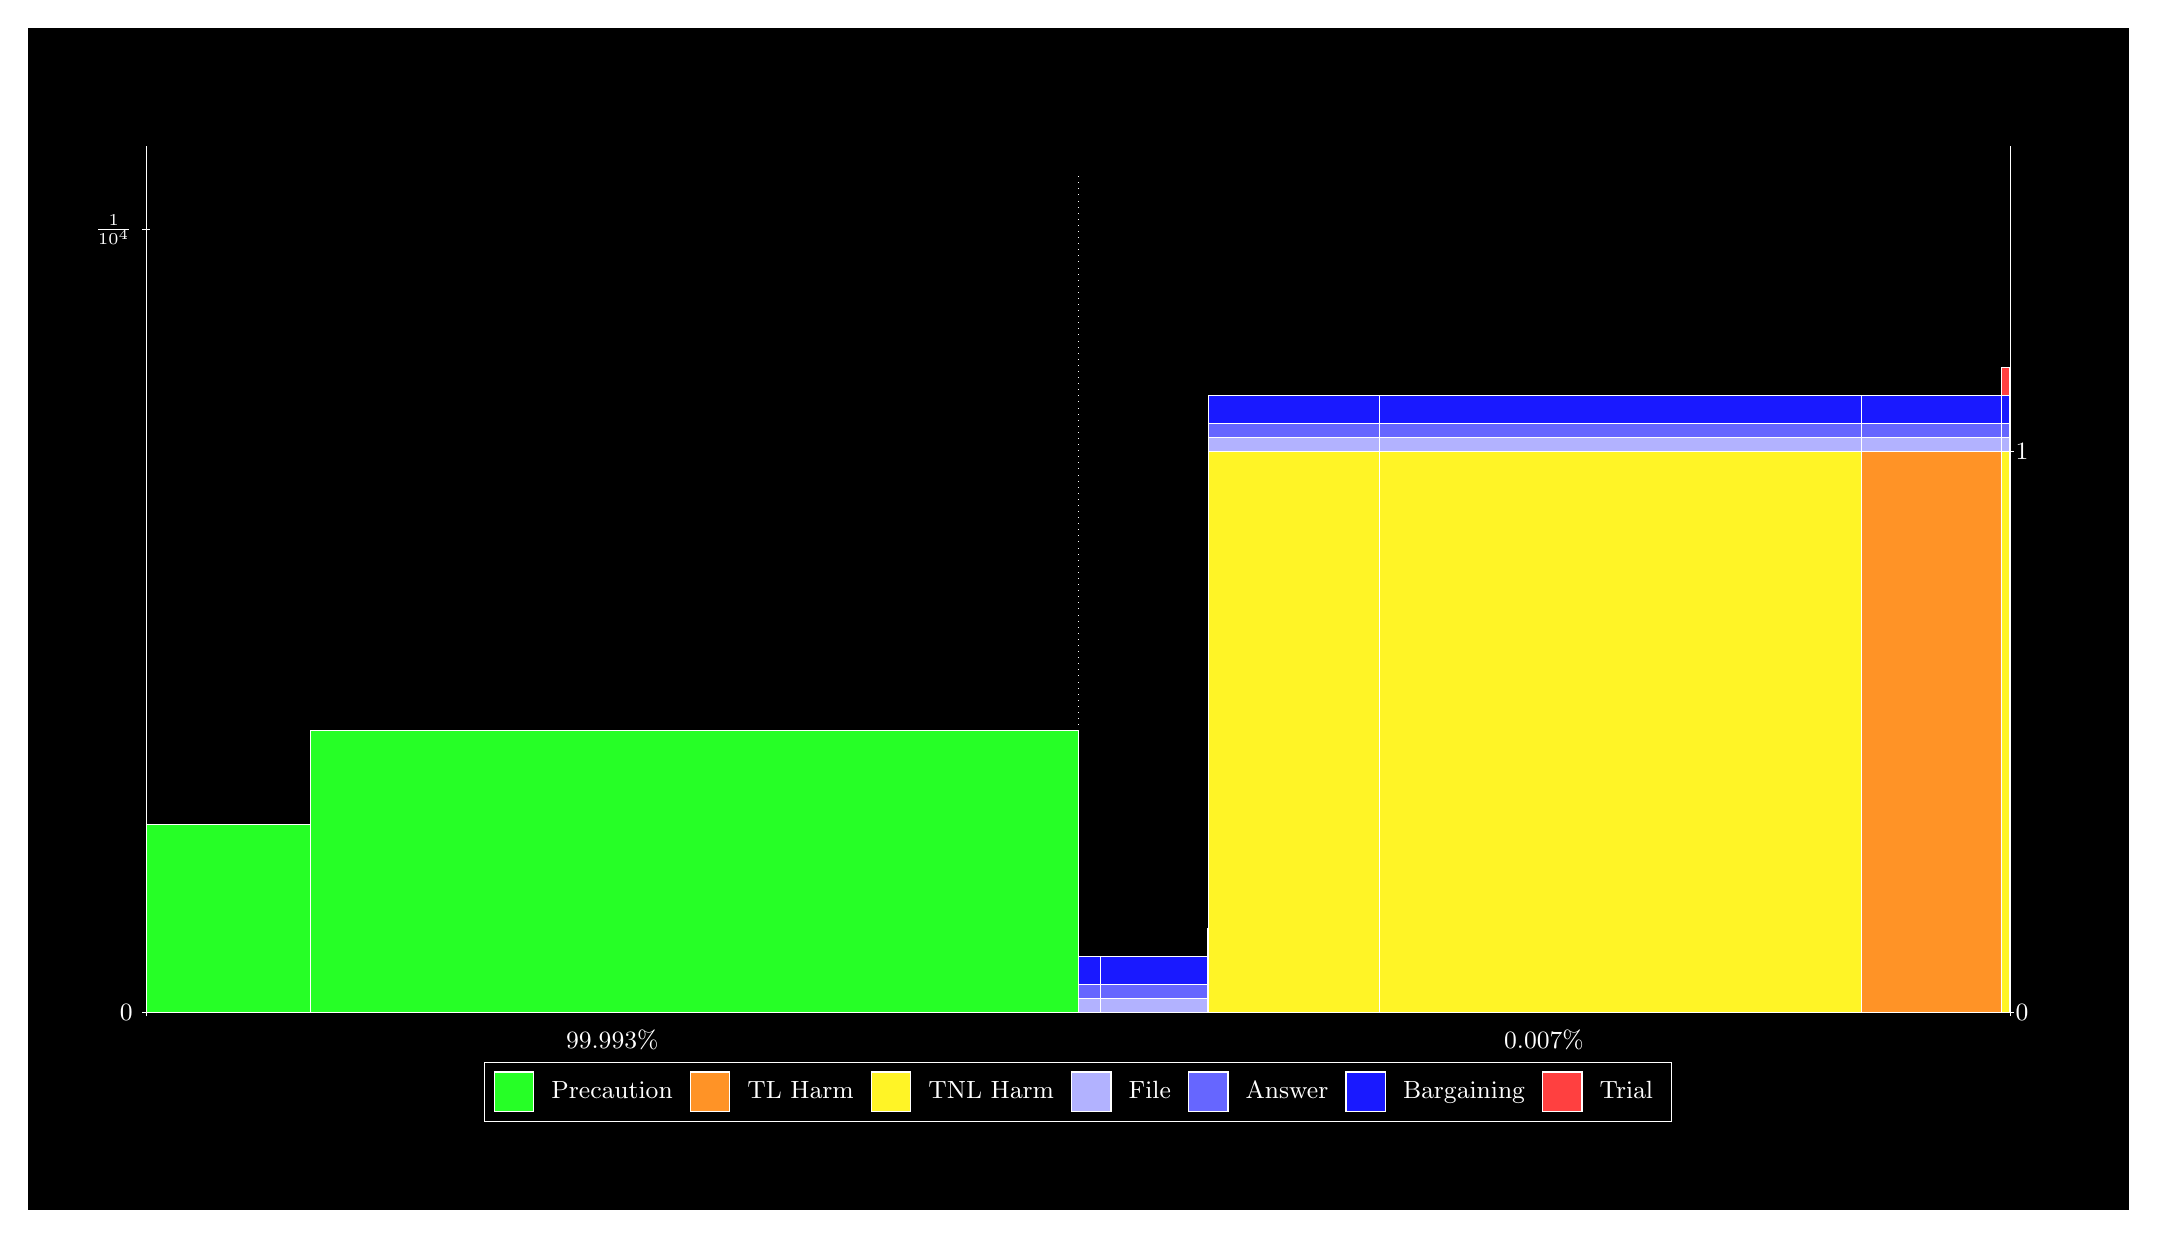
\begin{tikzpicture}
\draw[fill=black] (0,0) rectangle (26.667,15);
\draw[fill=green!85,draw=white,very thin] (1.5,2.5) rectangle (3.585,4.8866);
\draw[fill=green!85,draw=white,very thin] (3.585,2.5) rectangle (13.333,6.0799);
\draw[fill=green!85,draw=white,very thin] (13.333,2.5) rectangle (13.609,2.5002);
\draw[fill=blue!30,draw=white,very thin] (13.333,2.5002) rectangle (13.609,2.6784);
\draw[fill=blue!60,draw=white,very thin] (13.333,2.6784) rectangle (13.609,2.8566);
\draw[fill=blue!90,draw=white,very thin] (13.333,2.8566) rectangle (13.609,3.2129);
\draw[fill=green!85,draw=white,very thin] (13.609,2.5) rectangle (14.969,2.5003);
\draw[fill=blue!30,draw=white,very thin] (13.609,2.5003) rectangle (14.969,2.6784);
\draw[fill=blue!60,draw=white,very thin] (13.609,2.6784) rectangle (14.969,2.8566);
\draw[fill=blue!90,draw=white,very thin] (13.609,2.8566) rectangle (14.969,3.213);
\draw[fill=green!85,draw=white,very thin] (14.969,2.5) rectangle (14.984,2.5002);
\draw[fill=blue!30,draw=white,very thin] (14.969,2.5002) rectangle (14.984,2.6784);
\draw[fill=blue!60,draw=white,very thin] (14.969,2.6784) rectangle (14.984,2.8566);
\draw[fill=blue!90,draw=white,very thin] (14.969,2.8566) rectangle (14.984,3.2129);
\draw[fill=red!75,draw=white,very thin] (14.969,3.2129) rectangle (14.984,3.5693);
\draw[fill=green!85,draw=white,very thin] (14.984,2.5) rectangle (17.159,2.5002);
\draw[fill=yellow!85,draw=white,very thin] (14.984,2.5002) rectangle (17.159,9.6278);
\draw[fill=blue!30,draw=white,very thin] (14.984,9.6278) rectangle (17.159,9.806);
\draw[fill=blue!60,draw=white,very thin] (14.984,9.806) rectangle (17.159,9.9842);
\draw[fill=blue!90,draw=white,very thin] (14.984,9.9842) rectangle (17.159,10.341);
\draw[fill=green!85,draw=white,very thin] (17.159,2.5) rectangle (17.162,2.5002);
\draw[fill=orange!85,draw=white,very thin] (17.159,2.5002) rectangle (17.162,9.6278);
\draw[fill=blue!30,draw=white,very thin] (17.159,9.6278) rectangle (17.162,9.806);
\draw[fill=blue!60,draw=white,very thin] (17.159,9.806) rectangle (17.162,9.9842);
\draw[fill=blue!90,draw=white,very thin] (17.159,9.9842) rectangle (17.162,10.341);
\draw[fill=green!85,draw=white,very thin] (17.162,2.5) rectangle (23.284,2.5003);
\draw[fill=yellow!85,draw=white,very thin] (17.162,2.5003) rectangle (23.284,9.6279);
\draw[fill=blue!30,draw=white,very thin] (17.162,9.6279) rectangle (23.284,9.8061);
\draw[fill=blue!60,draw=white,very thin] (17.162,9.8061) rectangle (23.284,9.9843);
\draw[fill=blue!90,draw=white,very thin] (17.162,9.9843) rectangle (23.284,10.341);
\draw[fill=green!85,draw=white,very thin] (23.284,2.5) rectangle (25.053,2.5003);
\draw[fill=orange!85,draw=white,very thin] (23.284,2.5003) rectangle (25.053,9.6279);
\draw[fill=blue!30,draw=white,very thin] (23.284,9.6279) rectangle (25.053,9.8061);
\draw[fill=blue!60,draw=white,very thin] (23.284,9.8061) rectangle (25.053,9.9843);
\draw[fill=blue!90,draw=white,very thin] (23.284,9.9843) rectangle (25.053,10.341);
\draw[fill=green!85,draw=white,very thin] (25.053,2.5) rectangle (25.157,2.5002);
\draw[fill=yellow!85,draw=white,very thin] (25.053,2.5002) rectangle (25.157,9.6278);
\draw[fill=blue!30,draw=white,very thin] (25.053,9.6278) rectangle (25.157,9.806);
\draw[fill=blue!60,draw=white,very thin] (25.053,9.806) rectangle (25.157,9.9842);
\draw[fill=blue!90,draw=white,very thin] (25.053,9.9842) rectangle (25.157,10.341);
\draw[fill=red!75,draw=white,very thin] (25.053,10.341) rectangle (25.157,10.697);
\draw[fill=green!85,draw=white,very thin] (25.157,2.5) rectangle (25.167,2.5002);
\draw[fill=orange!85,draw=white,very thin] (25.157,2.5002) rectangle (25.167,9.6278);
\draw[fill=blue!30,draw=white,very thin] (25.157,9.6278) rectangle (25.167,9.806);
\draw[fill=blue!60,draw=white,very thin] (25.157,9.806) rectangle (25.167,9.9842);
\draw[fill=blue!90,draw=white,very thin] (25.157,9.9842) rectangle (25.167,10.341);
\draw[fill=red!75,draw=white,very thin] (25.157,10.341) rectangle (25.167,10.697);
\draw[white,very thin] (1.5,2.5) -- (1.5,13.5);
\draw[white,very thin] (1.45,2.5) -- (1.55,2.5);
\node[font=\small,text=white, anchor=east] at (1.45, 2.5) {0};
\draw[white,very thin] (1.45,12.444) -- (1.55,12.444);
\node[font=\small,text=white, anchor=east] at (1.45, 12.444) {$\frac{1}{10^{4}}$};

\draw[white,dotted,very thin] (13.333,2.83) -- (13.333,13.17);
\draw[white,very thin] (25.167,2.5) -- (25.167,13.5);
\draw[white,very thin] (25.117,2.5) -- (25.217,2.5);
\node[font=\small,text=white, anchor=west] at (25.117, 2.5) {0};
\draw[white,very thin] (25.117,9.6276) -- (25.217,9.6276);
\node[font=\small,text=white, anchor=west] at (25.117, 9.6276) {1};

\draw[white,very thin] (1.5,2.5) -- (25.167,2.5);
\draw[white,very thin] (1.5,2.45) -- (1.5,2.55);
\node[font=\small,text=white, anchor=north] at (1.5, 2.45) {};
\draw[white,very thin] (25.167,2.45) -- (25.167,2.55);
\node[font=\small,text=white, anchor=north] at (25.167, 2.45) {};

\node[font=\small,text=white,anchor=south] at (7.4167, 1.9) {99.993\%};
\node[font=\small,text=white,anchor=south] at (19.25, 1.9) {0.007\%};
\draw (13.3333,2.5) node (B) {};
\begin{scope}[align=center]
\matrix[scale=0.5,draw=white,below=0.5cm of B,nodes={draw},column sep=0.1cm]{
\node[rectangle,draw,minimum width=0.5cm,minimum height=0.5cm,fill=green!85]{}; & \node[draw=none,font=\small,text=white]{Precaution}; &
\node[rectangle,draw,minimum width=0.5cm,minimum height=0.5cm,fill=orange!85]{}; & \node[draw=none,font=\small,text=white]{TL Harm}; &
\node[rectangle,draw,minimum width=0.5cm,minimum height=0.5cm,fill=yellow!85]{}; & \node[draw=none,font=\small,text=white]{TNL Harm}; &
\node[rectangle,draw,minimum width=0.5cm,minimum height=0.5cm,fill=blue!30]{}; & \node[draw=none,font=\small,text=white]{File}; &
\node[rectangle,draw,minimum width=0.5cm,minimum height=0.5cm,fill=blue!60]{}; & \node[draw=none,font=\small,text=white]{Answer}; &
\node[rectangle,draw,minimum width=0.5cm,minimum height=0.5cm,fill=blue!90]{}; & \node[draw=none,font=\small,text=white]{Bargaining}; &
\node[rectangle,draw,minimum width=0.5cm,minimum height=0.5cm,fill=red!75]{}; & \node[draw=none,font=\small,text=white]{Trial}; \\\\
};\end{scope}

\end{tikzpicture}
\end{document}